\documentclass[border=5pt]{standalone} 
\usepackage{tikz}
\usetikzlibrary{bayesnet}
\usetikzlibrary{arrows}
\usepackage{amsmath}
\begin{document}
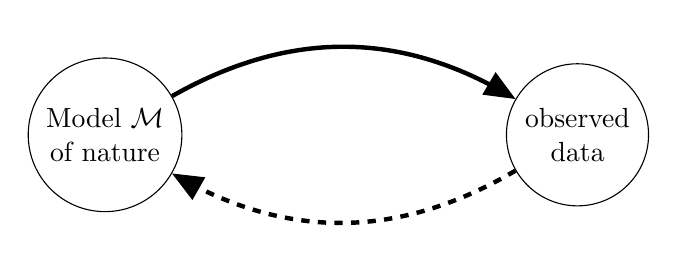
\begin{tikzpicture}
  \node[draw, circle, align=center] (nature) {Model $\mathcal{M}$ \\ of nature};
  \node[draw, circle, align=center, right of=nature, xshift=5cm] (data) {observed \\ data};
  \draw[->, ultra thick, bend left] (nature) to (data);
  \draw[->, dashed, ultra thick, bend left] (data) to (nature);
\end{tikzpicture}
\end{document}
